\documentclass[11pt,a4paper]{article}
%\documentclass[10pt,a4paper,aps,reprint,notitlepage]{revtex4-1}

\usepackage{graphicx}
\usepackage{enumitem}
\usepackage{amsmath}

\usepackage{phfcc}
%\usepackage[usemarginnote=false]{phfcc}

\phfMakeCommentingCommand[initials={PhF}]{phf}
\phfMakeCommentingCommand{jd}
\phfMakeCommentingCommand[initials={A.E.}]{AlE}
\phfMakeCommentingCommand{ccfour}
\phfMakeCommentingCommand{ccfive}
\phfMakeCommentingCommand{ccsix}
\phfMakeCommentingCommand[initials={cc7}]{ccseven}
\phfMakeCommentingCommand[initials={cc8}]{cceight}
\phfMakeCommentingCommand{ccnine}
\phfMakeCommentingCommand{ccten}



\begin{document}
\title{Document title}
\author{Me}
\begin{abstract}
  We characterize the work cost of state transitions using a framework based on
  Landauer's Principle and on the so-called noisy operations introduced
  by~[Horodecki et al, PRA, 2003]. Noisy operations correspond to adding a fully
  mixed ancilla, performing a unitary, and removing the ancilla. Previous work
  has demonstrated the relation between these operations and the mathematical
  notion of majorization.
\end{abstract}
\maketitle

\section{Introduction and Framework}

This example document contains some early material of mine which has been
suitably modified to test the functionalities of the present packages.

Landauer's Principle~\cite{Landauer1961_5392446Erasure}, and more generally the
\phf{relation between the second law of thermodynamics and information theory},
\jd*{has driven much attention} \jd has received tons of attention \endjd in the
past decades.  Studies have notably focused on heat generated by
computation~\cite{Bennett1982IJTP_ThermodynOfComp}, the exorcism of Maxwell's
demon via information theory (see eg.~\cite{Bennett2003_NotesLP}), and
generalizations to \AlE{quantum settings such as characterization of
  entanglement} through thermodynamical
considerations~\cite{Oppenheim2002PRL_thermodynamical}, \ccfour{or the
  determination of the single} shot work cost \ccfive{of the erasure of a
  quantum} \ccsix{system with quantum} side
\ccseven{information}~\cite{delRio2011Nature}.

\cceight{Some previous work has attempted to justify Landauer's Principle and
  generalizations} through explicit \ccnine{models such as Szilard
  boxes}~\cite{Szilard1929ZeitschriftFuerPhysik,Dahlsten2011NJP_inadequacy}, or
explicit Hamiltonian models~\cite{Alicki2004_hamiltonian}, all of which are NOT
depicted in \figurename~\ref{fig:test}. We will follow a different approach by
assuming Landauer's Principle as being valid, much like one generally accepts
the second law of thermodynamics as being valid. This allows us to {\em define}
a notion of work in our quantum setting by characterizing how much
\ccten{randomness can be absorbed or is generated} during a noisy
operation.\footnote{This is how a footnote looks like.} Yes.\footnote{Another
  footnote.} \ccsix![You might want to pay attention to this comment]

This notion is closely related to the notion of {\em themomajorization} introduced by
Horodecki et al.~\cite{Horodecki2013_ThermoMaj}. However, while their approach is to model
the thermodynamics of physical systems with more realistic non-degenerate Hamiltonians, we
adopt in contrast a purely information-theoretical point of view with degenerate
Hamiltonians and unitary computations.

\phf* You can comment entire chunks of text, like this:

Consider a quantum mechanical system $X$ in an inital state described by the
density operator $\sigma$.  Our task is to bring the system $X$ to another state
$\rho$, while attempting to maximize some kind of notion of ``extracted'' work
in the process.

The allowed operations are:
\begin{enumerate}[label=(\alph*)]
\item Bring the system $X$ (or an ancilla $A$) of $n$ qubits from any state to a pure state (`erasure') at
  cost $n\,kT\ln 2$ work;
\item Bring the system $X$ (or an ancilla $A$) of $n$ qubits from a pure state to a fully mixed state while
  extracting $n\,kT\ln 2$ work;
\item Add and remove ancillas in pure or fully mixed states at no work cost, as long as all the ancillas have
  been restored to their initial state at the end of the process;
\item Perform arbitrary unitaries (over $S$ and any added ancillas) at no work cost.
\end{enumerate}

and even equations:
\begin{equation}
  x = y^2\ .
\end{equation}
that's it! \endphf

\clearpage
Let's now start a new page to test a few things.

First, about footnotes. Let's check this out.%\footnote{\ifinner INNER\fi This: \ccnine{I wanna check if comments work in footnotes.}}  And minipages:
\\
\fbox{\begin{minipage}{4cm}
  We could try to {comment} in a \marginnote{footnote} %\footnote{\ccseven[like this!] :-)}
 to see what happens.  Hopefully everything won't immediately break
  down.  You might really need \texttt{\textbackslash marginnote} here, though.
\end{minipage}}\\
And equations:
\begin{equation}
  a + b = c \text{\jd{\(\displaystyle{}+O(x^2)\)}}
\end{equation}
And AMS equations:
\begin{align}
  a + b = c \text{\AlE{\(\displaystyle{}+O(x^2)\)}}
\end{align}

Now let's just check out Fig.~\ref{fig:test}.
\begin{figure}
  \centering
  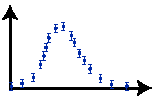
\includegraphics[width=4cm]{testfigure}
  \caption{This test figure is a test figure, for example to verify that the line spacing
    of captions is correct. Lorem ipsum test.  Uput non amet si dolor no voler a ponopodar
    esto gargantua.  Latinum no es ma specialitatum. \phf[A comment in figure caption]}
  \label{fig:test}
\end{figure}



\bibliographystyle{unsrt}
\bibliography{testnote.bibolamazi}

\end{document}

%%% Local Variables: 
%%% mode: latex
%%% TeX-master: t
%%% End: 
